\documentclass[12pt, a4paper]{article}
\usepackage[margin=1in]{geometry}
\usepackage[utf8x]{inputenc}
\usepackage{indentfirst} %indentace prvního odstavce
\usepackage{mathtools}
\usepackage{amsfonts}
\usepackage{amsmath}
\usepackage{amssymb}
\usepackage{graphicx}
\usepackage{enumitem}
\usepackage{subfig}
\usepackage{float}
\usepackage[czech]{babel}
\usepackage{mathdots}
\usepackage{slashbox}
\usepackage{braket}

\begin{document}
\begin{center}
\large Kvantová informace - zápočtové úlohy

\normalsize Jan Oupický
\end{center}
\vspace{1\baselineskip}

\section{}
idk

\section{}
Klasický SWAP vypadá takto:\\
\begin{center}
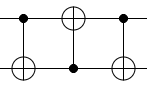
\includegraphics{2/swap.png}
\end{center}
Použítím této ekvivalence CNOT pomocí Hadamardových matic:\\
\begin{center}
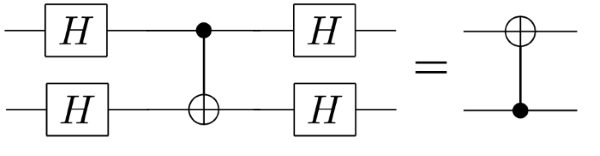
\includegraphics{2/hadamard.png}
\end{center}
se zbavíme prostředního CNOT, který je v jiném směru. Výsledný obvod je tedy:
\begin{center}
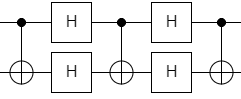
\includegraphics{2/final.png}
\end{center}

\section{}
Řešení je v principu spočítat AND prvního a druhého qubitu samostatně a zároveň stejně třetího a čtvrtého. A spočítat výsledný AND těchto výsledků, který je ekvivalentní ANDu všech 4 \uv{najednou}.

Použijeme tedy 3x CCNOT. Ten ale potřebujeme rozložit pomocí dvoukubitových bran. Použijeme postup ve skriptech, jak rozložit dvoukontrolovaný jednokubitový operátor na jednokontrolované jednokubitové. Použijeme tedy matici $X$ a spočítáme její odmocninu $\sqrt{X}$ a její hermitovsky sdruženou $\sqrt{X}^{-1}$. Matice jsou:
\begin{gather*}
X = \begin{pmatrix}
0 & 1\\
1 & 0
\end{pmatrix}, 
\sqrt{X} = \frac{1}{2}\begin{pmatrix}
1+i & 1-i\\
1-i & 1+i
\end{pmatrix},
\sqrt{X}^{-1} = \frac{1}{2}\begin{pmatrix}
1-i & 1+i\\
1+i & 1-i
\end{pmatrix}
\end{gather*}
Výsledný obvod tedy vypadá takto:
\begin{center}
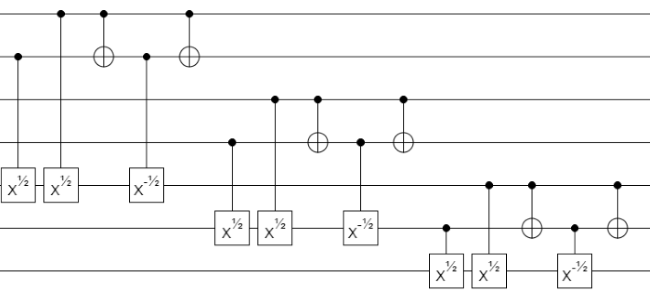
\includegraphics{3/AND.png}
\end{center}

První 4 dráty jsou vstupní 4 qubity. V 5. drátě je výsledek AND prvního a druhého, v 6. je 3. a 4. a v posledním se spočítá AND 5. a 6., což je požadovaný výsledek.

\section{}
Postupujeme dle skript. Pro 15 volíme $n=4$ a pro 21 $n=5$, v obou případěch $m=n$ (značí řád, který jistě $\leq n$). Obvod pro 21 se liší od 15 pouze počtem použitých drátů. Jako $a$ je v obou případech zvoleno $a=2$.

Obvod pro 15:
\begin{center}
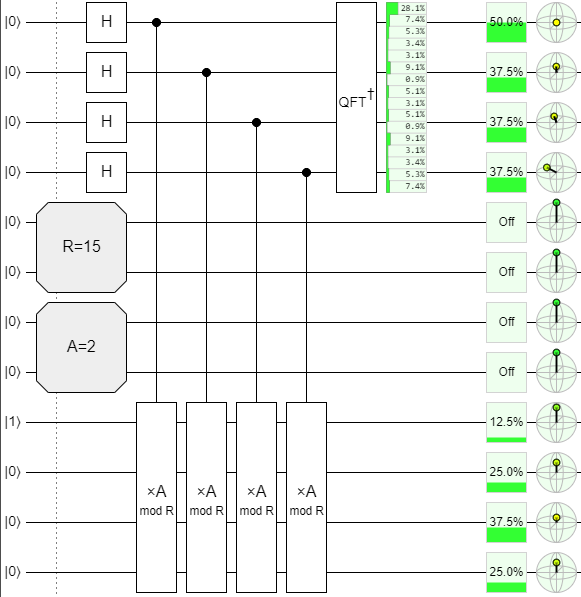
\includegraphics{4/15.png}
\end{center}\\
Obvod pro 21:
\begin{center}
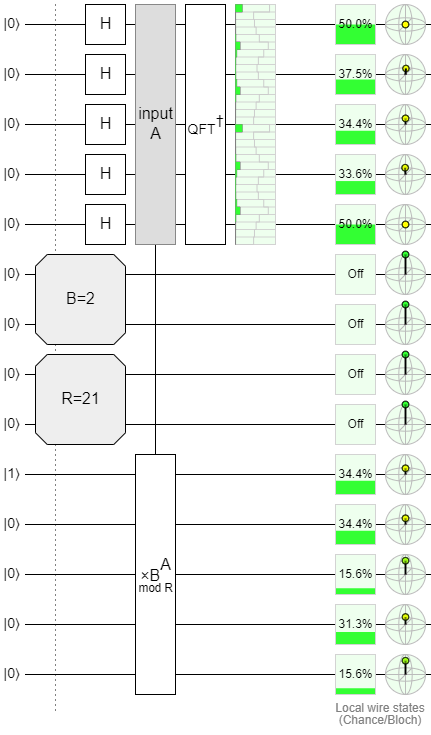
\includegraphics{4/21.png}
\end{center}

\section{}
Chceme $N$ t.ž. $\phi(N)=2^i, i \in \mathbb{N}$, protože $\phi(N)=|\mathbb{Z}^*_N|$. Předpokládáme, že $N$ je složené, liché a bezčtvercové. Tedy $N = p_1p_2\dots p_n, p_i\neq p_j$ pro $j\neq i$, zároveň z vlastností eulerovy funkce plyne, že $\phi(N)=\phi(p_1)\phi(p_2)\dots \phi(p_n) = (p_1-1)(p_2-1)\dots (p_n-1)=2^i$ neboli pro každé $p_i$ musí existovat $e_i \in \mathbb{N}$ t. ž. $p_i = 2^{e_i} + 1$. 

Hledáme tedy čísla, která jsou o jedno větší než nějaká mocnina $2$ a jsou prvočísla. Nalezl jsem: 3, 5, 17, 257. Dále je můžeme kombinovat díky vlastnostem uvedeným výše, máme tedy například čísla: $17\cdot 3 = \underline{51}$, $17 \cdot 5 = \underline{85}, 17 \cdot 5 \cdot 3 = \underline{255}$, $257\cdot 3 = \underline{771}$, $257 \cdot 5 = \underline{1285}$.

Vzhledem k otázce \uv{Kolik takových čísel existuje?} odpověď neznám. Prvočísla, která mají tvar $2^i + 1$, se nazývají Fermatova prvočísla a dle Wikipedie je jich známo pouze 5. Čísla co hledáme jsou právě všechny možné násobky těchto prvočísel, problémy tedy přímo souvisí, ale odpověď se asi neznámá v tuto chvíli.

\section{}
Dle přechozího cvičení víme, že $N = p_1p_2\dots p_n, p_i\neq p_j$ pro $j\neq i$, kde $\forall p_i \exists e_i \in \mathbb{N}: p_i = 2^{e_i}+1$. Zřejmě máme omezení na možná $e_i < \lfloor \log_2(N) \rfloor$. Algoritmus tedy vyzkouší všechny možné exponenty $e \in \mathbb{N}: e < \lfloor \log_2(N) \rfloor$  jejichž počet je omezen $\log(N)$, pro každý exponent spočítej $x \coloneqq \gcd(N,2^e+1)$, pokud $x=1$ inkrementuj $e$, pokud $x \neq 1$, tak máme faktor $N$, který je $2^e+1$.

Nechť $n = \log(N)$ (počet cifer $N$). Složitost je $n \cdot n^2$, kde $n$ je výše zmíněný počet kandidátů na $e$ a $n^2$ je složitost výpočtu GCD. Výsledná složitost je tedy $n^3$.

\section{}
Ze skript víme, jak udělat obvod, který \uv{proplete} 2 qubity. Obvod vypadá následovně:
\begin{center}
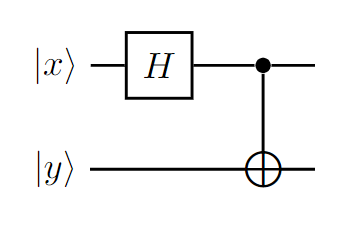
\includegraphics{7/hint.png}
\end{center}
Pokud $x = 0, y = 0$, tak dostaneme stav $\frac{\ket{00} + \ket{11}}{\sqrt(2)}$, který je propletený. Rozšířením obvodu o jeden CCNOT dostaneme stav $\frac{\ket{000}+\ket{111}}{\sqrt{2}}$, který si ukážeme, že je propletený.

Obvod tedy vypadá:
\begin{center}
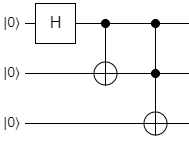
\includegraphics{7/circ.png}
\end{center}
Výpočet správnosti:
\begin{gather*}
\ket{0} \otimes \ket{0} \otimes \ket{0} \stackrel{H \otimes id \otimes id}{=} \frac{\ket{0}+\ket{1}}{\sqrt{2}} \otimes \ket{0} \otimes \ket{0} = \frac{\ket{00}+\ket{10}}{\sqrt{2}} \otimes \ket{0} \stackrel{CNOT \otimes id}{=} \frac{\ket{00}+\ket{11}}{\sqrt{2}} \otimes \ket{0} = \\
\frac{\ket{000}+\ket{110}}{\sqrt{2}} \stackrel{CCNOT}{=} \frac{\ket{000}+\ket{111}}{\sqrt{2}}
\end{gather*}

Dokážeme, že je to propletený stav. Ukážeme, že nelze napsat jako tenzorový součin vektorů z prostorů $\mathbb{H}_2$. BÚNO můžeme ignorovat $\frac{1}{\sqrt{2}}$ (normalizační faktor):
\begin{gather*}
a,b,c,d,e,f,g \in \mathbb{C}, (a\ket{0}+b\ket{1})\otimes(c\ket{0}+d\ket{1})\otimes(e\ket{0}+f\ket{1}) = ace\ket{000} + acf\ket{001} + ade\ket{010} + \\
adf\ket{011} + bce\ket{100} + bcf\ket{101} + bde\ket{110} + bdf\ket{111}
\end{gather*}
Abychom získali vektor $\ket{000}+\ket{111}$ musí platit: $ace \neq 0 \implies a\neq0, c\neq 0, e\neq 0 \land bdf \neq 0 \implies b\neq 0, d \neq 0, f \neq 0$. Potřebujeme ale nulové koeficienty u ostatních bázových vektorů což je spor, jelikož již předpokládáme, že všechny koeficienty jsou nenulové. Stav je tedy propletený.

\section{}
Postupujeme dle vzorce ze skript pro matici $X = \begin{pmatrix}
0 & 1 \\
1 & 0
\end{pmatrix}$. Nechť $\ket{\phi} = \begin{pmatrix} 2-i \\ i \end{pmatrix} \implies \ket{\phi}' \coloneqq \frac{\ket{\phi}}{\lVert \ket{\phi} \rVert} = \frac{1}{\sqrt{6}} \begin{pmatrix}
2-i \\ i 
\end{pmatrix}$.
\begin{gather*}
E(X) = \bra{\phi}' X \ket{\phi}' = \frac{1}{6} (2i + i^2 -2i + i^2) = \frac{-1}{3}
\end{gather*}

\section{}
Dle vzorce ze skript chceme spočítat $\bra{\phi} P_1 \ket{\phi}$. Ze zadání víme, jak bude vypadat $P_1$. Potřebujeme nejprve z daných vektorů udělat ON bázi, která je 
\begin{gather*}
b_1 = \frac{1}{\sqrt{2}}\begin{pmatrix}
1 \\
0 \\
0 \\
1
\end{pmatrix},
b_2 = \frac{1}{2} \begin{pmatrix}
1 \\
1 \\
1 \\
-1
\end{pmatrix} \implies P_1 = \ket{b_1}\bra{b_1} + \ket{b_2}\bra{b_2} \implies\\
P_1 = \begin{pmatrix}
\frac{3}{4} & \frac{1}{4} & \frac{1}{4} & \frac{1}{4} \\
\frac{1}{4} & \frac{1}{4} & \frac{1}{4} & \frac{-1}{4} \\
\frac{1}{4} & \frac{1}{4} & \frac{1}{4} & \frac{-1}{4} \\
\frac{1}{4} & \frac{-1}{4} & \frac{-1}{4} & \frac{3}{4}
\end{pmatrix}
\end{gather*}
Dále potřebujeme spočítat zadaný vektor jako prvek $\mathbb{H}_4$. To spočítáme pomocí vlastností tenzorového součinu:
\begin{gather*}
\begin{pmatrix}
1+i\\
i
\end{pmatrix} \otimes
\begin{pmatrix}
1-i\\
2i
\end{pmatrix} = ((1+i)\ket{0} + i\ket{1}) \otimes ((1-i)\ket{0} + 2i\ket{1}) = \\
(1+i)(1-i)\ket{00} + 2i(1+i)\ket{01} + i(1-i)\ket{10} + 2i^2\ket{11} = \\
2\ket{00} + (2i-2)\ket{01} + (1+i)\ket{10} - 2\ket{11} = 
\begin{pmatrix}
2\\
-2+2i\\
1+i\\
-2
\end{pmatrix} \stackrel{\text{znormování}}{\implies} \ket{\phi} \coloneqq \frac{1}{3\sqrt{2}}\begin{pmatrix}
2\\
-2+2i\\
1+i\\
-2
\end{pmatrix}
\end{gather*}
Výsledná pravděpodobnost se tedy spočítá:
\begin{gather}
\frac{1}{36}
\begin{pmatrix}
2 & -2-2i & 1-i & -2
\end{pmatrix} \begin{pmatrix}
\frac{3}{4} & \frac{1}{4} & \frac{1}{4} & \frac{1}{4} \\
\frac{1}{4} & \frac{1}{4} & \frac{1}{4} & \frac{-1}{4} \\
\frac{1}{4} & \frac{1}{4} & \frac{1}{4} & \frac{-1}{4} \\
\frac{1}{4} & \frac{-1}{4} & \frac{-1}{4} & \frac{3}{4}
\end{pmatrix} \begin{pmatrix}
2\\
-2+2i\\
1+i\\
-2
\end{pmatrix} = \frac{1}{4}
\end{gather}
\end{document}